% Options for packages loaded elsewhere
\PassOptionsToPackage{unicode}{hyperref}
\PassOptionsToPackage{hyphens}{url}
\PassOptionsToPackage{dvipsnames,svgnames*,x11names*}{xcolor}
%
\documentclass[
]{article}
\usepackage{amsmath,amssymb}
\usepackage{lmodern}
\usepackage{ifxetex,ifluatex}
\ifnum 0\ifxetex 1\fi\ifluatex 1\fi=0 % if pdftex
  \usepackage[T1]{fontenc}
  \usepackage[utf8]{inputenc}
  \usepackage{textcomp} % provide euro and other symbols
\else % if luatex or xetex
  \usepackage{unicode-math}
  \defaultfontfeatures{Scale=MatchLowercase}
  \defaultfontfeatures[\rmfamily]{Ligatures=TeX,Scale=1}
\fi
% Use upquote if available, for straight quotes in verbatim environments
\IfFileExists{upquote.sty}{\usepackage{upquote}}{}
\IfFileExists{microtype.sty}{% use microtype if available
  \usepackage[]{microtype}
  \UseMicrotypeSet[protrusion]{basicmath} % disable protrusion for tt fonts
}{}
\makeatletter
\@ifundefined{KOMAClassName}{% if non-KOMA class
  \IfFileExists{parskip.sty}{%
    \usepackage{parskip}
  }{% else
    \setlength{\parindent}{0pt}
    \setlength{\parskip}{6pt plus 2pt minus 1pt}}
}{% if KOMA class
  \KOMAoptions{parskip=half}}
\makeatother
\usepackage{xcolor}
\IfFileExists{xurl.sty}{\usepackage{xurl}}{} % add URL line breaks if available
\IfFileExists{bookmark.sty}{\usepackage{bookmark}}{\usepackage{hyperref}}
\hypersetup{
  pdftitle={Catch Subtitution between Coastal Pelagic Species under Climate Change Scenarios},
  pdfauthor={Felipe Quezada1,2,},
  colorlinks=true,
  linkcolor=Maroon,
  filecolor=Maroon,
  citecolor=Blue,
  urlcolor=blue,
  pdfcreator={LaTeX via pandoc}}
\urlstyle{same} % disable monospaced font for URLs
\usepackage[margin=1in]{geometry}
\usepackage{graphicx}
\makeatletter
\def\maxwidth{\ifdim\Gin@nat@width>\linewidth\linewidth\else\Gin@nat@width\fi}
\def\maxheight{\ifdim\Gin@nat@height>\textheight\textheight\else\Gin@nat@height\fi}
\makeatother
% Scale images if necessary, so that they will not overflow the page
% margins by default, and it is still possible to overwrite the defaults
% using explicit options in \includegraphics[width, height, ...]{}
\setkeys{Gin}{width=\maxwidth,height=\maxheight,keepaspectratio}
% Set default figure placement to htbp
\makeatletter
\def\fps@figure{htbp}
\makeatother
\setlength{\emergencystretch}{3em} % prevent overfull lines
\providecommand{\tightlist}{%
  \setlength{\itemsep}{0pt}\setlength{\parskip}{0pt}}
\setcounter{secnumdepth}{5}
\usepackage{mathtools} \usepackage{tcolorbox} \usepackage{float} \floatplacement{figure}{H} \usepackage{times} \usepackage{setspace} \setstretch{1.5}
\usepackage{booktabs}
\usepackage{longtable}
\usepackage{array}
\usepackage{multirow}
\usepackage{wrapfig}
\usepackage{float}
\usepackage{colortbl}
\usepackage{pdflscape}
\usepackage{tabu}
\usepackage{threeparttable}
\usepackage{threeparttablex}
\usepackage[normalem]{ulem}
\usepackage{makecell}
\usepackage{xcolor}
\ifluatex
  \usepackage{selnolig}  % disable illegal ligatures
\fi
\usepackage[]{natbib}
\bibliographystyle{plainnat}

\title{Catch Subtitution between Coastal Pelagic Species under Climate
Change Scenarios}
\author{Felipe Quezada\textsuperscript{1,2,*}}
\date{November 1, 2021}

\begin{document}
\maketitle
\begin{abstract}
Fisher do not only catch one species. They have a set of possible
choices, called `fishing portfolio' and allow them to diversify as a way
to reduce income risk. Some species are easier to shift as gear and
method used are similar between them. Therefore, the cost of shifting
between species is low and fishers could adapt quickly to a shift in
fish species spatial distributions in response to climate change.
Nevertheless, it is not clear whether actually this substitution happen
as other constraint may be in play. Port constraints, as well as market
characteristics and regulation could reduce substitution between
species. In this study we analyze how changing in spatial distribution
and the closure of Pacific sardine fishery affects landing subtitution
between three coastal pelagic species: Pacific sardine, market squid and
Northern anchovy. Moreover, we study how spatial distribution and
closure affects vessels participation decisions in the CPS fishery using
a discrete choice modelling approach. We use species distribution
projection to see how landings and participations change under different
future climate change scenarios.
\end{abstract}

\textsuperscript{1} Institute of Marine Sciences, University of
California Santa Cruz\\
\textsuperscript{2} NOAA Southwest Fisheries Science Center

\textsuperscript{*} Correspondence:
\href{mailto:felipe.quezada@noaa.gov}{Felipe Quezada
\textless{}\href{mailto:felipe.quezada@noaa.gov}{\nolinkurl{felipe.quezada@noaa.gov}}\textgreater{}}

\hypertarget{introduction}{%
\section{Introduction}\label{introduction}}

Fishing portfolios are an important mechanism to safeguard fishers
livelihood. Diversification strategy have been principally associated to
reducing income variability \citep{kasperski2013}. For instance, when a
species abundance is reduced due to environmental conditions, fisher can
change the targeted species to one that requires similar gears. However,
there is no always room for diversification. Switching between species
can be costly if gears are quite different between species, or a new
permit is required for legal fishing. Moreover, even though fisher may
have flexibility switching between species, port infrastructure and
markets may impose some restrictions on this flexibility, as well as
regulations that limits access to fisheries to avoid collapse of fish
stocks from overfishing \citep{kasperski2013}. Therefore, it is not
clear how change in species distribution and regulation would be
reflected in landings compositions and participation.

In this study we analyze how changing in spatial distribution as well as
the implementation of a fishery's closure affects landing and fisher
participation of three coastal pelagic species (CPS) harvested in U.S.
West Coast: Pacific sardine (PSDN), market squid (MSQD) and Northern
anchovy (NANC). Fisheries closures are a interesting policy instrument
in a multispecies framework as give us the opportunity to study a
quasi-experiment. However, fewer studies have study the effect of one
fishery closure in other fishery outcomes. SOme examples are
\citet{vermard2008} study the effect of an anchovy closure in trip
choices conducted by the Bay of Biscai pelagic fleet, and
\citet{richerson2017} who study the effect of salmon closures in vessel
participation on salmon fishery, but also in other fisheries. In this
paper, we study the effect of the 2015 Pacific sardine closure
implemented after the overxplotation of the fishery. The answer to this
questions is not straightforward as different response can be observed
to the same conditions as fishers and vessel are heterogeneous
\citep{zhang2011}. Moreover, we have to consider that species are
interconnected, at least economically if not ecologically, so a
multispecies framework that considering interrelation between them is
necessary. Our research give a step further and analyze the CPS as a
multispecies fishery. This is in line with recent literature that start
to consider multiple species in their analysis \citep{richerson2017}.
Our goal is to understand how changing in species distribution and
closure of Pacific sardine affect vessel responses in landing amount and
participation, the substitution between species, and to what extent
future projected climate will affect landings, catch composition and
participation of fishers.

Our papers builds on the model developed by \citet{smith2021potential}
for sardine landings. We expand their model including a landing equation
for all of the three species analyzed and estimating a multilevel
Bayesian model in order to incorporate heterogeneity between fleets and
ports. Moreover, we use the probability of presence obtained from
Species Distribution Models (SDM) as explanatory variable instead of
landing by species. This allows us to project landing over time using
SDM predictions for different climate scenarios. We analyze how species
distribution interact between each others. We expect that this additions
allows us to characterize better how fishers portfolio is composed, and
also to understand better species interactions on catch rates.
Additionally, we also estimate a multiple species participation model
based on \citet{richerson2017} who study the effect of salmon closure on
annual fishers participation, expanding their analysis to the CPS
fishery in monthly basis, allowing to understand seasonality within
fishing season. For this, we develop a Random Utility Model (RUM) to
model monthly vessel participation in targeting a specific species in
the CPS fishery as a function of\ldots{} \textbf{fisher characteristics
including revenue level, diversification, dependence on the species and
spatial variables of area and range..}

The remainder of the paper is organized as follows: Section
\ref{coastal-pelagic-species-fishery} provides background on the CPS
fishery in the US west coast. In Section \ref{methods} we discusses our
data set and empirical strategy. Section \ref{results} presents the
results of the estimations, and we conclude in Section
\ref{conclusions}.

\hypertarget{coastal-pelagic-species-fishery}{%
\section{Coastal Pelagic Species
fishery}\label{coastal-pelagic-species-fishery}}

Before Pacific sardine closure in 2015, landings in the CPS fishery have
been mainly dominated by Pacific sardine and market squid, as is shown
in panel (a) in Figure \ref{fig:avg_lan_rev}. Low average landings for
Pacific herring and Northern anchovy could be related with geography and
regulatory constraint that restrict vessels to exploit them.
Nevertheless, this lower levels compare with Market squid and Pacific
sardine could be reflecting lower economics incentives for its
exploitation. In terms of revenue, we can observe in panel (b) that
market squid have the largest revenue, while Pacific sardine lost
relevance due to the low prices received by fishers.

\begin{figure}
\centering
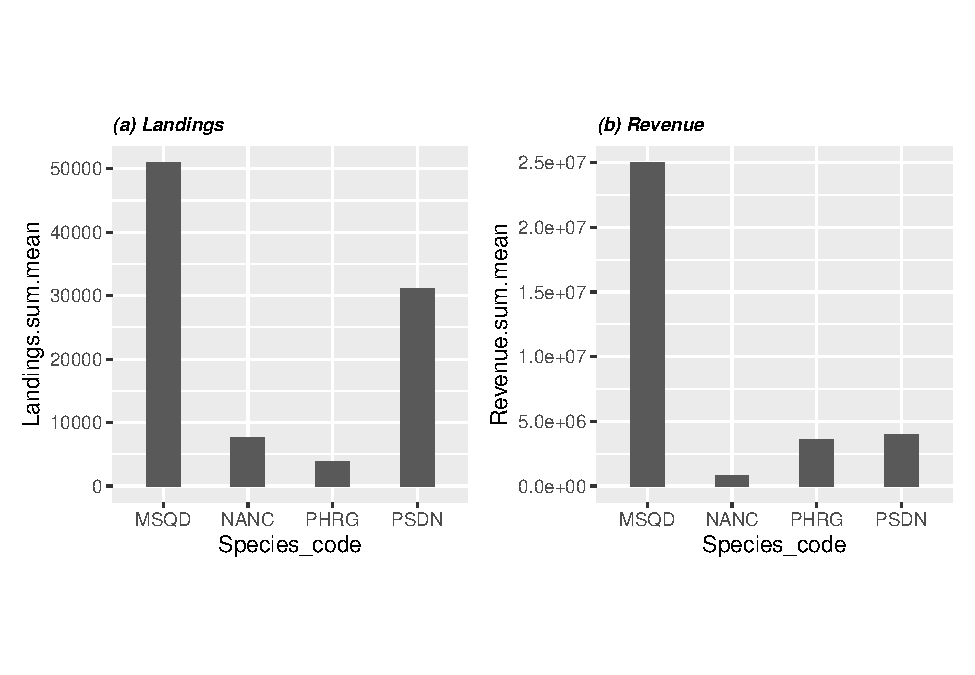
\includegraphics{econ_landings_paper_files/figure-latex/avg_landings-1.pdf}
\caption{Average annual landing and revenues for the CPS fishery by
species.\label{fig:avg_lan_rev}}
\end{figure}

Landings composition varies geographically. We show in Figure
\ref{fig:avg_landings_by_ports} average annual landings by ports areas.
We can observe that market squid is mostly landed in the southern ports
located in Los Angeles, Santa Barbara and Monterrey areas, while Pacific
sardine is mainly landed in Los Angeles and Monterrey areas in
California, and also in the Columbia river area in Oregon. Substitution
between species seems to be more likely in Los Angeles, Monterrey and
Santa Barbara area ports (and in some lower scale at San Francisco area)
as positive values for market squid, Pacific sardine and Northern
anchovy landings are observed.

\begin{figure}
\centering
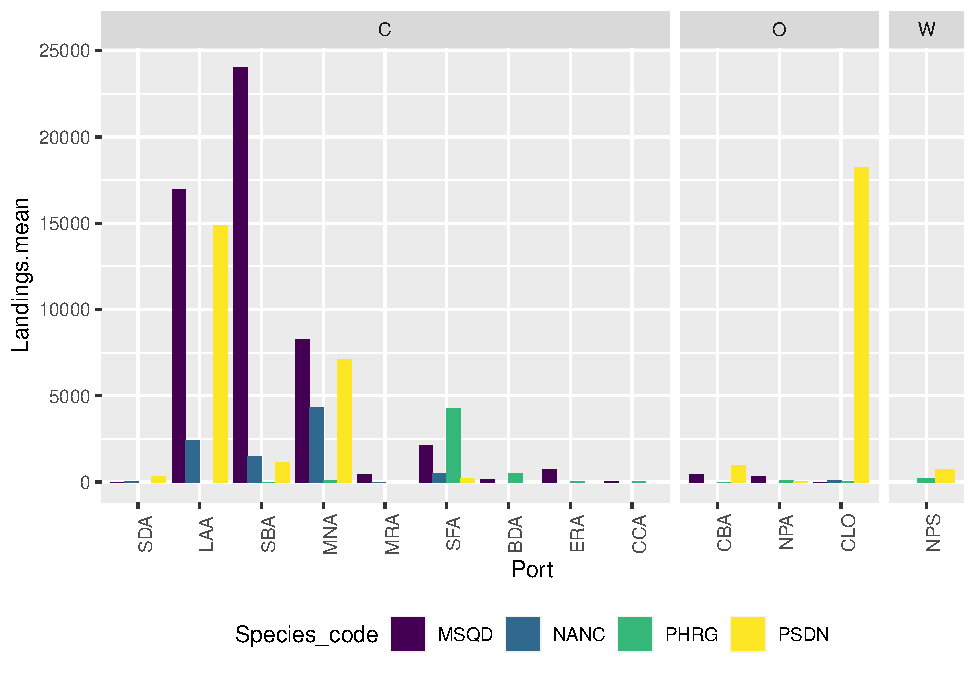
\includegraphics{econ_landings_paper_files/figure-latex/avg_landings_by_port-1.pdf}
\caption{Annual average landings by port
area.\label{fig:avg_landings_by_ports}}
\end{figure}

To analyze substitution more in detail, we compute total annual landing
by port during 1980-2020 period (Figure \ref{fig:ts_landings_by_ports}).
There is a general conception that vessel that harvest Pacific sardine
switch to market squid when the conditions are favorable. However, we
can notice from Figure \ref{fig:ts_landings_by_ports} that landings of
market squid have been decreasing in the last five years. We would
expect that the closure of the Pacific sardine fishery would have switch
targeted species, but the graphs show some complementary instead of
substitution. Under this scenario is useful to ask to ask whether after
the closure, vessel that harvest Market squid left the fishery or
stayed, which we can answer from our multispecies participation model.
We show the number of vessels by species in Figure
\ref{fig:ts_n_vessels}. This would be suggesting an unintended
consequence from a policy that aims to only affect Pacific sardine, but
its effect affects indirectly other fisheries \citep{richerson2017}.

\begin{figure}
\centering
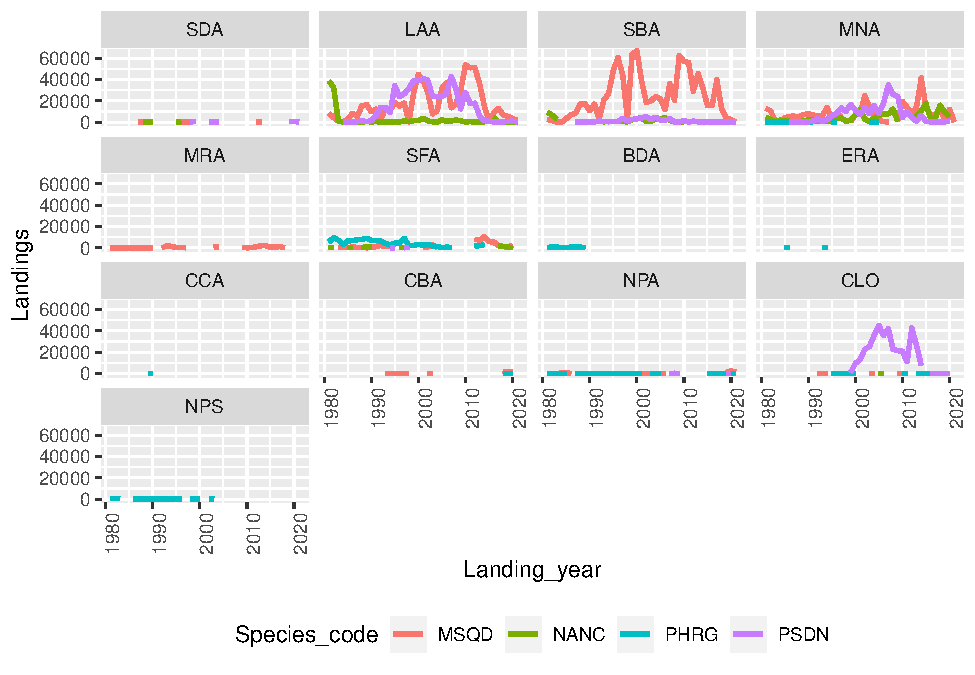
\includegraphics{econ_landings_paper_files/figure-latex/ts_by_port-1.pdf}
\caption{Total annual landing by port area. 2000 - 2020. \textit{Notes:}
CLO = Columbia River (OR); LAA = Los Angeles; MNA = Monterey; SBA =
Santa Barbara; SFA = San Francisco.\label{fig:ts_landings_by_ports}}
\end{figure}

\begin{figure}
\centering
\includegraphics{econ_landings_paper_files/figure-latex/ts_by_port_price-1.pdf}
\caption{Total annual landing by port area. 2000 - 2020. \textit{Notes:}
CLO = Columbia River (OR); LAA = Los Angeles; MNA = Monterey; SBA =
Santa Barbara; SFA = San Francisco.\label{fig:ts_price_by_ports}}
\end{figure}

\begin{figure}
\centering
\includegraphics{econ_landings_paper_files/figure-latex/ts_n_vessels-1.pdf}
\caption{Total number of vessel by species. 2000 -
2020.\label{fig:ts_n_vessels}}
\end{figure}

\textbf{\textless\textless{} SHOULD WE STUDY HOW FISHING GROUNDS CHANGE
FROM PORTS (THUS DISTANCE TO FISHING GROUNDS AND WEATHER VARIABLES
AFFECTED), LIKE SELDEN (2020) AND PAPAIOANNOU (2021)??? IN BOTH MODELS?
\textgreater\textgreater{}}

\hypertarget{methods}{%
\section{Methods}\label{methods}}

\hypertarget{multispecies-landing-model}{%
\subsection{Multispecies Landing
Model}\label{multispecies-landing-model}}

Our data set contain a number of variables measured at the port and
\emph{vessel levels} for CPS the fishery located in the U.S. West Coast.
In regard to landings, our outcome variables are landings by port areas
in a year, landing by vessel in a month. These two different outcome
variables would allows us to study the degree of flexibility that vessel
have in comparison to ports in regard to species substitution and catch
composition. If vessels have strong contracts with processor associated
with a port, then we should observe that substitution of vessels and
port is similar. Yearly panel data data on landing by port areas during
the the period 1980 - 2020 is publicly available from
\href{http://pacfin.psmfc.org/}{PacFIN}. \textbf{Vessel level data was
obtained upon request from\ldots{}} We only include ports areas where
substitution could happen. In practical terms, we drop port that have
never landed either Pacific sardine, market squid or Northern anchovy
during our period of analysis.\footnote{N/A were converted to zero.} We
assume that this criteria would allows to identify ports that have the
infrastructure to land all of the species in consideration.

Our main treatment variables are species probability of presence and
Pacific sardine closure. Probability of presence were obtained from
Species Distribution Models (SDM), and future forecast of these
variables allows us to simulate the CPS fishery in the future.
Distribution of species have change relative to ports in the last
decades \citep{selden2020}. Thus, it have been used to explain
variability in fish landings
\citep[\citet{smith2021potential}]{selden2020}. For instance,
\citet{smith2021potential} use mean monthly probability of presence of
sardine within 60 km of the port as explanatory variable. They found a
positive effect of probability of presence on Pacific sardine landings.
Moreover, landings where mostly explained by this variable. We follow
their same procedure to associate SDM's outputs with ports. For Pacific
sardine, we compute the average probability of presence within the same
radius of 60 kilometers around the port. This radius also coincide with
the average distance with two standard deviation traveled by vessels
based on logbooks available for these fisheries.\footnote{\citet{selden2020}
  use the 75th quantile of the travel distances made by vessels to
  define the availability of an species associated to a port for
  multiple species, and weight this distances by the catch of those
  species.} For market squid and Northern anchovy, we set this radius to
90 and 20 kilometers, respectively, also based in the average distance
to fishing ground obtained from logbooks.\footnote{To see an animation
  of how far vessel travel please visit
  \href{https://drive.google.com/file/d/1-PE_lcZNcXNcyILA_6xhkHyEhV3mV2TA/view?usp=sharing}{this
  link}.}

Figure \ref{fig:sdm_land_by_port} show the relationship between the
probability of presence and landings by species in three main port
areas: Los Angeles, Monterrey and Santa Barbara areas. The graph suggest
that Pacific sardine landings are positive correlated with the
probability of presence of this species, similar to
\citet{smith2021potential}. This is also true in Monterrey area for the
Northern anchovy, In the case of market squid, we cannot distinguish
correlation between landings and probability of presence. Note, however,
that the evidence shown in this figure may not capturing the actual
effect of the probability of presence as other effect may be in play.
Our empirical strategy is designed to isolate the effect of the
probability on landing in a multivariate model framework.

\begin{figure}
\centering
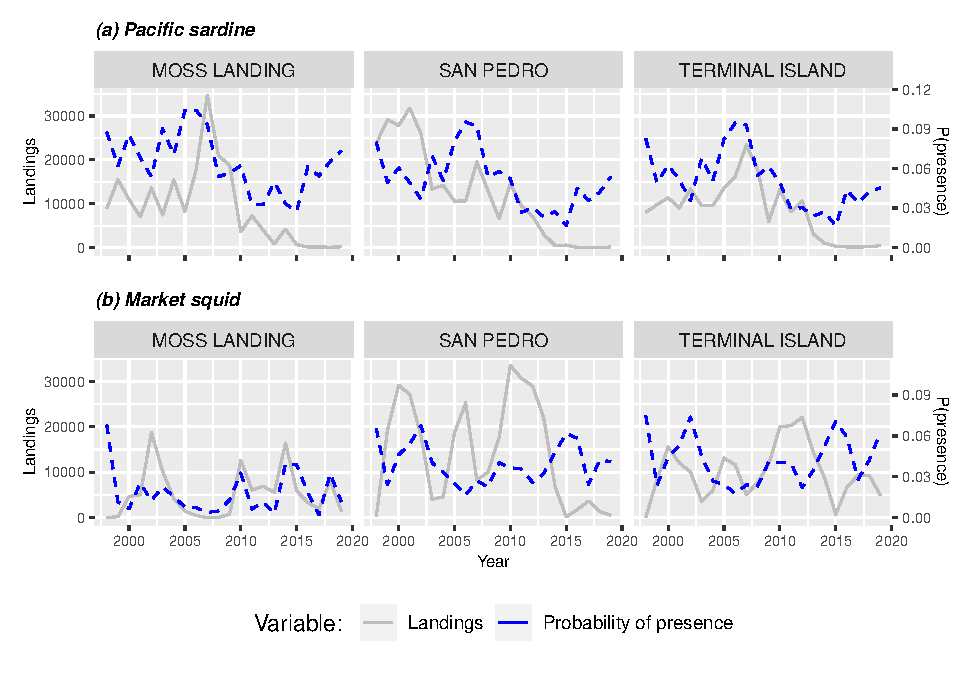
\includegraphics{econ_landings_paper_files/figure-latex/SDM_land_by_port-1.pdf}
\caption{Landings v/s probability of presence by port area.
\textit{Notes:} LAA = Los Angeles; MNA = Monterey; SBA = Santa
Barbara.\label{fig:sdm_land_by_port}}
\end{figure}

We use a Hierarchical Bayesian Hurdle model to estimate the effect of
species distribution on fish landings. We estimate a separate model for
the three species in consideration. We use a Bayesian framework for
several reasons. First, it allows us to consider uncertainty from
modeling the process as well as from the imperfect observation of the
process, assuming that all parameters are random variables. Second, it
allows us to incorporate multilevel effects (i.e.~hierarchical effects).
Finally, it allow us to incorporate previous knowledge as a prior. For
instance, we can include a prior the results obtained in
\citet{smith2021potential} for the Pacific sardine landing equation.

Specifically, we fit a hierarchical Bayesian hurdle model to model the
zeros included in our landing data. We observe a zero when no landings
occur in a specific time period (landings observations with ``NA'' were
transformed to zero). This zero could mean that there was no incentives
for the fleet/vessel to harvest the species in consideration. In
general, our Bayesian models have the following structure:
\begin{align*}
[\theta_i | q_{it}] &  \varpropto f\left(q_{it} | \theta_i\right) \times [\theta_i] 
\end{align*} where \(q_{it}\) is the observed landings of the
corresponding species in port \(i \in (1,\ldots,L)\) at year \(t\),
\(L\) is the total number of port, and \(\theta_i\) are the parameters
(i.e.~random-coefficients) to be estimated at the port level. The latter
give the name of hierarchical to our model.\footnote{For more details
  about Hierarchichal models, see \cite{hobbs2015}.} The distribution
\(f\left(q_{it} | \theta_i\right)\) can be rewritten as:
\begin{equation}
f\left(q_{it} | \theta_i \right) = \begin{cases}
p_{it} & \text{if} \quad q_{it} = 0  \\ 
\left[1-p_{it}\right] \text{gamma_i} \left(q_{it} | \frac{\mu_{it}^2}{\sigma^2}, \frac{\mu_{it}}{\sigma^2} \right) & \text{if} \quad q_{it} > 0. 
\end{cases}
\end{equation} where \(\text{logit}(p_{it}) = \bf{X}\gamma_i\) and
\(\mu_{it} = \bf{X}\beta_i\). Specifically \(\mu_{it}\) is defined as
the following: \begin{equation}
\mu_{it} = \beta_{0,i} + \beta_{1,i} P(Precense.PSDN)_{it} + \beta_{2,i} + P(Precense.MSQD)_{it} + \beta_{3,i} P(Precense.NANC)_{it}.
\end{equation} \(\text{logit}(p_{it})\) follows the same structure, but
coefficient \(\beta_i\) are replaced by \(\gamma_i\).

Beside the biological stock, landings are affected by socio-economics
conditions. Some of them are harvest cost, prices received by species
and their substitutes, and regulations imposed by the authorities. In
our data we include as a proxy of harvest cost average distances
traveled by vessel from the port of origin \emph{(TO BE INCLUDED USING
GLOBAL FISHING WATCH\ldots)} and fuel cost \emph{(TO BE
INCLUDED\ldots)}. Own price was included and it was obtained from PacFIN
landings dataset. When price was missing, we replace this value for the
average price of the species in all ports for the corresponding year.

We include the Annual Catch Limit (ACL) for the Pacific sardine model as
an additional explanatory variable in both \(\mu_i\) and
\(\text{logit}(p_i)\) equations. ACL variable is the total quota
allocated each year for this fishery and was obtained from the
\href{pcouncil.org}{CPS Fisheries Management Plan}???. For this species,
we restrict our data set to the period when the fishery was open
(2000-2015). We only consider ports where landing have occur at least
once in our sample period. Thus, we avoid to deal with ports where
infrastructure to land Pacific sardine is nonexistent.

\begin{table}[!htbp] \centering \renewcommand*{\arraystretch}{1.1}\caption{Summary Statistics \label{tab:sum_stats}}\resizebox{\textwidth}{!}{
\begin{tabular}{lrrrrrrr}
\hline
\hline
Variable & N & Mean & Std. Dev. & Min & Pctl. 25 & Pctl. 75 & Max \\ 
\hline
Landings: PSDN & 92 & 10828.886 & 13499.627 & 0.1 & 156.025 & 20991.3 & 45016.5 \\ 
Landings: MSQD & 103 & 13383.623 & 17166.411 & 0.1 & 222.2 & 19693.75 & 66890.3 \\ 
Landings: NANC & 59 & 2769.698 & 3928.055 & 0 & 149.55 & 3651.65 & 17180.2 \\ 
Prob(presence): PSDN & 322 & 0.261 & 0.104 & 0.08 & 0.177 & 0.341 & 0.569 \\ 
Prob(presence): MSQD & 280 & 0.17 & 0.078 & 0.025 & 0.12 & 0.217 & 0.467 \\ 
Prob(presence): NANC & 308 & 0.499 & 0.175 & 0.176 & 0.349 & 0.623 & 0.914 \\ 
Price: PSDN & 437 & 0.079 & 0.039 & 0 & 0.05 & 0.108 & 0.37 \\ 
Price: MSQD & 437 & 0.266 & 0.121 & 0 & 0.185 & 0.32 & 0.5 \\ 
Price: NANC & 437 & 0.091 & 0.054 & 0 & 0.06 & 0.114 & 0.35 \\ 
Revenue: PSDN & 92 & 1497414 & 1920819.177 & 0 & 31471 & 2646660.75 & 8979099 \\ 
Revenue: MSQD & 103 & 7734746.485 & 9938728.985 & 0 & 97348 & 11193641.5 & 43742173 \\ 
Revenue: NANC & 59 & 311373.814 & 427339.961 & 17 & 42203 & 437046.5 & 1930490 \\ 
Annual Catch Limit: PSDN & 436 & 82613.151 & 55614.651 & 0 & 30259 & 122747 & 186791\\ 
\hline
\hline
\end{tabular}
}
\end{table}

In the case of market squid, our database comprise the time period
between 2000 and 2018. We do not include ACL as an explanatory variable
as there is no variation between years. To capture any change on fishers
behavior when Pacific sardine fishery closed, we include a binary
variable called \textbf{dClose} that takes the value ``1'' when the
Pacific sardine fishery is close, and the value ``0'' when its close.
Pacific sardine probability takes the value of zero when the fishery is
closed. Thus, the effect of this variable is only relevant when it
Pacific sardine fishery is open in order to capture potential
substitution between targets. Finally, a similar structure than Market
squid models is followed for our estimation of Northern anchovy landing
by ports. A summary statistics of our data set is shown in Table
\ref{tab:sum_stats}.

\hypertarget{multispecies-participation-model}{%
\subsection{Multispecies participation
model}\label{multispecies-participation-model}}

For the multispecies participation model, we follow a similar
methodology than \citet{richerson2017}. We estimate a discrete choice
model for probability that a vessel participate in a particular species
fishery during a specific month. This approach allows us to further
understand how a closure or abrupt weather/abundance changes restructure
fisher's portfolios.

In the participation model, our outcome variable is a categorical
variable that indicate whether a vessel participate in a specific
fishery. It ranges from 0 to 4 where: 0 = ``No fishing during the
month'', 1 = ``Pacific sardine'', 2 = ``Market Squid'', 3 = ``Northern
Anchovy'', and 4 = ``Other''. \textbf{\textless\textless Can I combine
Anchovy + sardine in category 5? What if in the same month a vessel
harvest two different species. Should we maybe assume 1 for the
principal species, zero to the second one?\textgreater\textgreater{}}
\textbf{\textless\textless{} We can use the approach of metier, where a
choice is created from data (see Andersen, 2012, ICES). Here would be a
combination of target species\textgreater\textgreater{}}
\textbf{\textless{}\textgreater{}} To select vessels in or database,
they should met the following criteria:

\begin{enumerate}
\def\labelenumi{\arabic{enumi}.}
\tightlist
\item
  Vessel active at least \textbf{XX\%} of the sample.
\item
  Total revenue at least \textbf{XX\%} of CPS fishery.
\item
  Total annual revenue average for two or more species listed of at
  least \textbf{XXX}.
\end{enumerate}

We expect that using monthly \textbf{\textless\textless Should I use
Yearly data???\textgreater\textgreater{}} data allows us to observe
seasonality in fishers´ behavior and to reduce the risk to not loosing
general behavior when we dissagregate data in a finer scale.

According \citet{richerson2017}, fishers participation decision should
depend, in general terms, on profitability, species distribution and
regulations. Specifically, based on different studies
\citep{richerson2017} (MORE REF), variables that can explain fishery
participation on a particular fishery in a month are:

\begin{itemize}
\tightlist
\item
  Previous revenues
\item
  Expected catch:

  \begin{itemize}
  \tightlist
  \item
    We calculate expected revenue as a function of average outputs of
    the SDMs. Using SDM outputs instead of catch to compute expected
    revenues allow us to project fishers decision on time using SDM's
    projections. Moreover, using catch to compute expected revenue as a
    regress in a discrete choice model could incorporate endogeneity as
    it can be correlated with unobservables not captured by the choice
    constant.
  \end{itemize}
\item
  Closure: Whether or not the Pacific sardine fishery was closed.
\item
  Diversification using HHI (measurement of diversification, from
  \citet{richerson2017})
\item
  Dependence on the species in consideration (historical \% of the
  revenue from the species considered)
\item
  Typical landings location: Latitudinal center of gravity (LCG) index
  from \citep{richerson2017}
\item
  Dispersion around centre of gravity: Latitude inertia (LI) index from
  \citep{richerson2017}
\item
  Years in the sample that the vessel have participate in the fishery.
\end{itemize}

We model the probability \(p_{ijm}\) that vessel \(i\) fishes species
\(j\) in month \(y\) as: \begin{align*}
\text{logit}(p_{ijy}) = & \beta_1 + \beta_2  Closure + \beta_3 Mean.revenue_j + \beta_4 ExpectedCatch_j \\
& + \beta_5 HHI_i + \beta_6 Percent.revenue_j + \beta_7 LCG_i + \beta_8 LI_i + \beta_9 Year.fished. 
\end{align*} Note that we are not able to observe if a vessel leave the
CPS fishery for another resource or actually exit fishing entirely.
Therefore, the outside option include is interpreted as ``No fishing in
any of the CPS fishery''.

Should we study also the desicion to leave or stay the CPS fishery? I
think in implicit in the participation model. Can we test this using the
prediction from that model?

\hypertarget{effort-susbsitution}{%
\subsection{Effort susbsitution}\label{effort-susbsitution}}

\begin{itemize}
\tightlist
\item
  Time series of number of trips (as a proxy for effort) for all the
  species
\item
  \citet{richerson2017} use a method identify the nature of the outliers
  in an ARMA time series model (read more if interested)

  \begin{itemize}
  \tightlist
  \item
    I propose to estimate a system of simultaneous equations (VECM
    model) to study equilibrium of effort and short-run and long-run
    effects of the closure (structural breaks)
  \item
    Have a long-run equation for each species (simultaneously estimated)
    and test for structural break in this long-run relationship.
  \end{itemize}
\end{itemize}

\hypertarget{seasonality-changes}{%
\subsection{Seasonality changes}\label{seasonality-changes}}

\begin{itemize}
\tightlist
\item
  Seasonality can be studied calculating monthly share of total trips by
  species, regress it using month dummiues and see any is there any
  structural change after the closure \citep{richerson2017}.
\end{itemize}

\hypertarget{results}{%
\section{Results}\label{results}}

\hypertarget{landing-model}{%
\subsection{Landing model}\label{landing-model}}

\hypertarget{graphical-posterior-predictive}{%
\subsubsection{Graphical posterior
predictive}\label{graphical-posterior-predictive}}

Before presenting the results for the three species in consideration, we
check graphically whether the posterior distribution is able to predict
the actual distribution. We exclude zero in our graph to avoid plotting
different data generation processes. In Figure \ref{fig:posteriors} we
show a posterior sample compare with the true sample distribution for
the three species in analysis. Some deviation from the true sample
distribution is observed in the three models, but still the posterior
sample follow a similar shape than the actual curve. Moreover, our
pacific sardine sample do well in predicting probabilities at lower
landing levels.

\begin{figure}
\centering
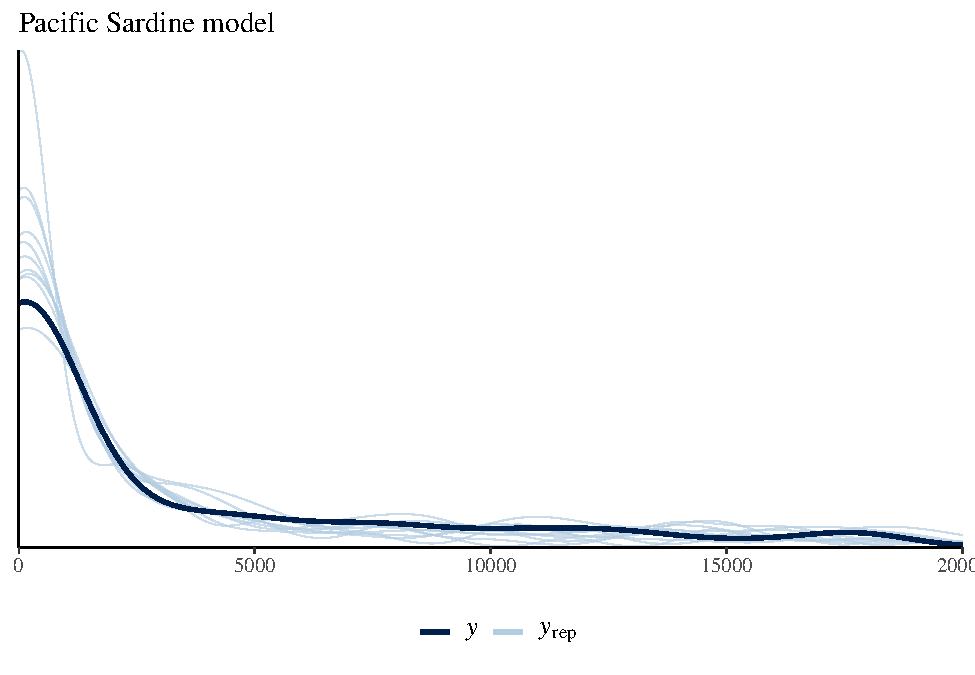
\includegraphics{econ_landings_paper_files/figure-latex/y_rep-1.pdf}
\caption{Graphical posterior predictive checks\label{fig:posteriors}}
\end{figure}

In addition to a posterior predictive check, we also check divergence
and treedepth.\footnote{Explain what are these concepts\ldots{}} In all
three models, we did not have any divergent step in our estimation. The
maximum treedepth was 11 for the Pacific sardine model, while in the
others it was 10.

\hypertarget{own-species-distribution-effect}{%
\subsubsection{Own species distribution
effect}\label{own-species-distribution-effect}}

The inclusion of hierarchical effects by port allows us to analyze the
effects of the probability of presence on landings disaggregated by
ports. We only focus our analysis in owns probability of presence
effects, as other probability are analyzed as interaction (see next
subsection). We can observe in Figure \ref{fig:sdmeffects} that the
effects of the own probability of presence on landings are not strong
(maybe I should use logs\ldots). However, it is clear that it have a
positive effect on landings, specially on port areas such as Columbia
River at Oregon for Pacific sardine, and Monterrey for Northern anchovy,
while a more moderate effect is observed at Santa Barbara Area for
Northern anchovy.

\begin{figure}
\centering
\includegraphics{econ_landings_paper_files/figure-latex/by_port_sdm-1.pdf}
\caption{Effect of probability of presence on landings by species and
port\label{fig:sdmeffects}}
\end{figure}

\hypertarget{interaction-effects}{%
\subsubsection{Interaction effects}\label{interaction-effects}}

To study the effect of other species distribution on landings, we
compute the conditional effects of the interaction between probabilities
of presence. Let denote species A the species which we are analysing its
landings, and species B and C the other species included in the model
for species A landings. For each species, we compute the effect on
landing of the interaction between the probability of presences of: +
Species A and species B, + Species A versus species C, + Species B
versus species C. For example, for the Pacific sardine equation, we
compute these results for the probability of presence effect between
Pacific sardine and market squid, Pacific sardine and Northern anchovy,
and market squid and Northern anchovy.

Let first analyze the interaction effect of the probability of presences
on Pacific sardine landings, presented in Figure \ref{fig:sdm_int_psdn}.
We only shows results for the main three port where Pacific sardine is
landed (Columbia River at Oregon, Los Angeles Area and Monterrey Area).
As we already commented in Figure \ref{fig:sdmeffects}, the effects the
Pacific sardine's own probability of presence is positive, changing
color from left to right in panels (a) and (b). Market squid seems to be
an stronger substitute for Pacific sardine than Northern anchovy. This
is suggested by the different slopes between panel (a) and panel (b).
For instane, in Columbia River, an increase in the probability of
presence for anchovy does decrease Pacific sardine landings as much as
an increase in the probability of presece of market squid.

\begin{figure}
\centering
\includegraphics{econ_landings_paper_files/figure-latex/int_effect_PSDN_by_port_PLOT-1.pdf}
\caption{Interaction effects between species distribution on Pacific
sardine landings by port\label{fig:sdm_int_psdn}}
\end{figure}

We found some similar findings for market squid in Figure
\ref{fig:sdm_int_msqd}. Pacific sardine it is a strong substitute of
market squid. In regard to Norther anchovy, there is some
complementarity with market squid. We observe that when Northern anchovy
presence increase, there is also an increase in market squid landings.

\begin{figure}
\centering
\includegraphics{econ_landings_paper_files/figure-latex/int_effect_MSQD_by_port_PLOT-1.pdf}
\caption{Interaction effects between species distribution on market
squid landings by port\label{fig:sdm_int_msqd}}
\end{figure}

However, this complementary is not observed for Northern anchovy
landings. When market squid presence increase, we observe a decrease in
Northern anchovy landings. An interesting case is observed for Pacific
sardine and Northern anchovy, in particular at Monterrey area. For small
levels of Pacific sardine presence, Pacific sardine is a complement with
Northern anchovy. However, after certain threshold, Pacific sardine is
no longer complement and Pacific sardine become a substitute, reducing
Northern anchovy landings when the probability of presence for Pacific
sardine increase.

\begin{figure}
\centering
\includegraphics{econ_landings_paper_files/figure-latex/int_effect_NANC_by_port_PLOT-1.pdf}
\caption{Interaction effects between species distribution on Northern
anchovy landings by port\label{fig:sdm_int_nanc}}
\end{figure}

\hypertarget{pacific-sardine-closure}{%
\subsubsection{Pacific sardine closure}\label{pacific-sardine-closure}}

Finally, lets analyze the effect of the Pacific sardine closure on
market squid and Northern anchovy landings. We do not find significant
results in the case of Northern anchovy. In the case of market squid, we
found a decrease in the level of landing after the closure was
implemented. It seems that some fisher exit the CPS fishery after the
closure of Pacific sardine, reducing their participation in the market
squid fishery. Our participation model results give us more details
about what happen after the Pacific sardine closure.

\begin{figure}
\centering
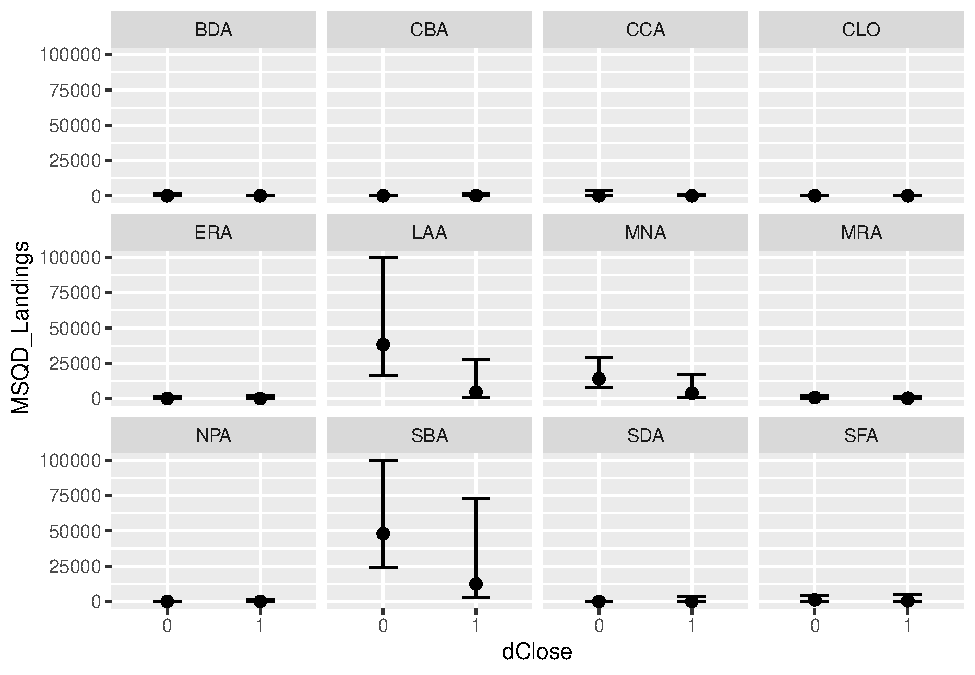
\includegraphics{econ_landings_paper_files/figure-latex/by_port_msqd_dclose-1.pdf}
\caption{Effect of Pacific sardine fishery closure on markt squid
landings by species and port\label{fig:sdmeffects}}
\end{figure}

\hypertarget{multispecies-participation-model-1}{%
\subsection{Multispecies participation
model}\label{multispecies-participation-model-1}}

\hypertarget{predictions}{%
\section{Predictions}\label{predictions}}

\ldots{}

\hypertarget{conclusions}{%
\section{Conclusions}\label{conclusions}}

A possible extension of our research is to consider spatial
autocorrelations between ports.\footnote{See \cite{morris2019bayesian}
  for an application of a spatial model in a Bayesian framework.} Ports
landing maybe correlated as vessel have the incentives to choose the
port of landing, conditional on whether the port have the infrastructure
for this. It is likely that they just land wherever is closer to the
area they are fishing. Nevertheless, differential in prices could
encourage them to travel a little further for higher prices.

  \bibliography{references.bib}

\end{document}
